% Options for packages loaded elsewhere
\PassOptionsToPackage{unicode}{hyperref}
\PassOptionsToPackage{hyphens}{url}
%
\documentclass[
]{book}
\usepackage{lmodern}
\usepackage{amssymb,amsmath}
\usepackage{ifxetex,ifluatex}
\ifnum 0\ifxetex 1\fi\ifluatex 1\fi=0 % if pdftex
  \usepackage[T1]{fontenc}
  \usepackage[utf8]{inputenc}
  \usepackage{textcomp} % provide euro and other symbols
\else % if luatex or xetex
  \usepackage{unicode-math}
  \defaultfontfeatures{Scale=MatchLowercase}
  \defaultfontfeatures[\rmfamily]{Ligatures=TeX,Scale=1}
\fi
% Use upquote if available, for straight quotes in verbatim environments
\IfFileExists{upquote.sty}{\usepackage{upquote}}{}
\IfFileExists{microtype.sty}{% use microtype if available
  \usepackage[]{microtype}
  \UseMicrotypeSet[protrusion]{basicmath} % disable protrusion for tt fonts
}{}
\makeatletter
\@ifundefined{KOMAClassName}{% if non-KOMA class
  \IfFileExists{parskip.sty}{%
    \usepackage{parskip}
  }{% else
    \setlength{\parindent}{0pt}
    \setlength{\parskip}{6pt plus 2pt minus 1pt}}
}{% if KOMA class
  \KOMAoptions{parskip=half}}
\makeatother
\usepackage{xcolor}
\IfFileExists{xurl.sty}{\usepackage{xurl}}{} % add URL line breaks if available
\IfFileExists{bookmark.sty}{\usepackage{bookmark}}{\usepackage{hyperref}}
\hypersetup{
  pdftitle={Screen Pixel Ruler {[}master{]}},
  pdfauthor={Stewart Cossey},
  hidelinks,
  pdfcreator={LaTeX via pandoc}}
\urlstyle{same} % disable monospaced font for URLs
\usepackage{color}
\usepackage{fancyvrb}
\newcommand{\VerbBar}{|}
\newcommand{\VERB}{\Verb[commandchars=\\\{\}]}
\DefineVerbatimEnvironment{Highlighting}{Verbatim}{commandchars=\\\{\}}
% Add ',fontsize=\small' for more characters per line
\usepackage{framed}
\definecolor{shadecolor}{RGB}{248,248,248}
\newenvironment{Shaded}{\begin{snugshade}}{\end{snugshade}}
\newcommand{\AlertTok}[1]{\textcolor[rgb]{0.94,0.16,0.16}{#1}}
\newcommand{\AnnotationTok}[1]{\textcolor[rgb]{0.56,0.35,0.01}{\textbf{\textit{#1}}}}
\newcommand{\AttributeTok}[1]{\textcolor[rgb]{0.77,0.63,0.00}{#1}}
\newcommand{\BaseNTok}[1]{\textcolor[rgb]{0.00,0.00,0.81}{#1}}
\newcommand{\BuiltInTok}[1]{#1}
\newcommand{\CharTok}[1]{\textcolor[rgb]{0.31,0.60,0.02}{#1}}
\newcommand{\CommentTok}[1]{\textcolor[rgb]{0.56,0.35,0.01}{\textit{#1}}}
\newcommand{\CommentVarTok}[1]{\textcolor[rgb]{0.56,0.35,0.01}{\textbf{\textit{#1}}}}
\newcommand{\ConstantTok}[1]{\textcolor[rgb]{0.00,0.00,0.00}{#1}}
\newcommand{\ControlFlowTok}[1]{\textcolor[rgb]{0.13,0.29,0.53}{\textbf{#1}}}
\newcommand{\DataTypeTok}[1]{\textcolor[rgb]{0.13,0.29,0.53}{#1}}
\newcommand{\DecValTok}[1]{\textcolor[rgb]{0.00,0.00,0.81}{#1}}
\newcommand{\DocumentationTok}[1]{\textcolor[rgb]{0.56,0.35,0.01}{\textbf{\textit{#1}}}}
\newcommand{\ErrorTok}[1]{\textcolor[rgb]{0.64,0.00,0.00}{\textbf{#1}}}
\newcommand{\ExtensionTok}[1]{#1}
\newcommand{\FloatTok}[1]{\textcolor[rgb]{0.00,0.00,0.81}{#1}}
\newcommand{\FunctionTok}[1]{\textcolor[rgb]{0.00,0.00,0.00}{#1}}
\newcommand{\ImportTok}[1]{#1}
\newcommand{\InformationTok}[1]{\textcolor[rgb]{0.56,0.35,0.01}{\textbf{\textit{#1}}}}
\newcommand{\KeywordTok}[1]{\textcolor[rgb]{0.13,0.29,0.53}{\textbf{#1}}}
\newcommand{\NormalTok}[1]{#1}
\newcommand{\OperatorTok}[1]{\textcolor[rgb]{0.81,0.36,0.00}{\textbf{#1}}}
\newcommand{\OtherTok}[1]{\textcolor[rgb]{0.56,0.35,0.01}{#1}}
\newcommand{\PreprocessorTok}[1]{\textcolor[rgb]{0.56,0.35,0.01}{\textit{#1}}}
\newcommand{\RegionMarkerTok}[1]{#1}
\newcommand{\SpecialCharTok}[1]{\textcolor[rgb]{0.00,0.00,0.00}{#1}}
\newcommand{\SpecialStringTok}[1]{\textcolor[rgb]{0.31,0.60,0.02}{#1}}
\newcommand{\StringTok}[1]{\textcolor[rgb]{0.31,0.60,0.02}{#1}}
\newcommand{\VariableTok}[1]{\textcolor[rgb]{0.00,0.00,0.00}{#1}}
\newcommand{\VerbatimStringTok}[1]{\textcolor[rgb]{0.31,0.60,0.02}{#1}}
\newcommand{\WarningTok}[1]{\textcolor[rgb]{0.56,0.35,0.01}{\textbf{\textit{#1}}}}
\usepackage{longtable,booktabs}
% Correct order of tables after \paragraph or \subparagraph
\usepackage{etoolbox}
\makeatletter
\patchcmd\longtable{\par}{\if@noskipsec\mbox{}\fi\par}{}{}
\makeatother
% Allow footnotes in longtable head/foot
\IfFileExists{footnotehyper.sty}{\usepackage{footnotehyper}}{\usepackage{footnote}}
\makesavenoteenv{longtable}
\usepackage{graphicx,grffile}
\makeatletter
\def\maxwidth{\ifdim\Gin@nat@width>\linewidth\linewidth\else\Gin@nat@width\fi}
\def\maxheight{\ifdim\Gin@nat@height>\textheight\textheight\else\Gin@nat@height\fi}
\makeatother
% Scale images if necessary, so that they will not overflow the page
% margins by default, and it is still possible to overwrite the defaults
% using explicit options in \includegraphics[width, height, ...]{}
\setkeys{Gin}{width=\maxwidth,height=\maxheight,keepaspectratio}
% Set default figure placement to htbp
\makeatletter
\def\fps@figure{htbp}
\makeatother
\setlength{\emergencystretch}{3em} % prevent overfull lines
\providecommand{\tightlist}{%
  \setlength{\itemsep}{0pt}\setlength{\parskip}{0pt}}
\setcounter{secnumdepth}{-\maxdimen} % remove section numbering
\usepackage{booktabs}
\usepackage{amsthm}
\makeatletter
\def\thm@space@setup{%
  \thm@preskip=8pt plus 2pt minus 4pt
  \thm@postskip=\thm@preskip
}
\makeatother
\usepackage[]{natbib}
\bibliographystyle{plainnat}

\title{Screen Pixel Ruler {[}master{]}}
\author{Stewart Cossey}
\date{2021-12-08}

\begin{document}
\maketitle

{
\setcounter{tocdepth}{1}
\tableofcontents
}
\hypertarget{overview}{%
\chapter{Overview}\label{overview}}

Screen Pixel Ruler is a on screen ruler that can assist in measuring elements from web pages, documents or software which does not implement a native ruler.
Based on .NET Core 3.1 and inspired by MioPlanet PixelRuler, this software is supported on Windows 7 and higher.

This software is free and open source; licensed under the \href{https://opensource.org/licenses/BSD-3-Clause}{BSD 3-Clause License}.

\hypertarget{features}{%
\section{Features}\label{features}}

\begin{itemize}
\tightlist
\item
  Global hotkeys to trigger functionality when other software is in focus.
\item
  Rotatable vertical or horizontal ruler. \texttt{Ctrl\ +\ Shift\ +\ Alt\ +\ R}
\item
  Customizable ruler themes.
\item
  Freezable position. \texttt{Ctrl\ +\ Shift\ +\ Alt\ +\ F}
\item
  Guideline system that can lock the mouse cursor horizontally or vertically
\item
  Position 0 of the ruler to the current cursor location. \texttt{Ctrl\ +\ Shift\ +\ Alt\ +\ S}
\end{itemize}

\begin{quote}
A list of all shorcuts can be found \protect\hyperlink{keyboard}{here}.
\end{quote}

\hypertarget{installation}{%
\section{Installation}\label{installation}}

Screen Pixel Ruler can be installed from either the \href{https://github.com/Cossey/ScreenPixelRuler2/releases}{Installer} or via \href{https://chocolatey.org}{Chocolatey Package Management} by running the command \texttt{choco\ install\ screenpixelruler}.
Both the installer and package will install the .NET Core 3.1 runtime if it is not present.

\hypertarget{providing-feedback}{%
\section{Providing feedback}\label{providing-feedback}}

You can report bugs or request features by opening an issue on the \href{https://github.com/Cossey/ScreenPixelRuler2}{GitHub repository}.
Any contributions are also welcome and can be done by creating a pull request.

\hypertarget{ui}{%
\chapter{User Interface}\label{ui}}

The user interface consists of a single ruler that can be displayed either horizontally or vertically.

\begin{figure}
\centering
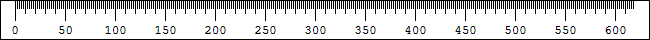
\includegraphics{images/ruler.png}
\caption{\label{fig:unnamed-chunk-1}The ruler user interface.}
\end{figure}

Holding down the primary mouse button on the ruler will allow you to drag the ruler around the screen.
Pressing the secondary mouse button on the ruler will display a context menu called the \emph{Ruler Menu}.

If the mouse cursor moves past the right or bottom edge of the ruler, it will automatically extend.
The ruler will stay extended if the cursor is frozen or if a Guideline has been set beyond the default size.
Guidelines are covered in further detail in the \protect\hyperlink{guidelines}{Guidelines} section.

\begin{quote}
The primary mouse button is determined by the \emph{Select your primary button} option in the \emph{Mouse Settings} in Microsoft Windows.
Typically it is the left mouse button.
\end{quote}

\hypertarget{rotate}{%
\section{Rotating the ruler}\label{rotate}}

The ruler can be rotated using the \texttt{Ctrl\ +\ Shift\ +\ Alt\ +\ R} key combination or by the \texttt{Ruler\ Menu\ →\ Rotate} menu item.
This is assignable to a mouse button click via the \texttt{Rotate} function.
It is not possible to have both a vertical and a horizontal ruler displayed at the same time.
When rotating the ruler, the axis changes but any \protect\hyperlink{guidelines}{Guidelines} are kept in the same position.

\hypertarget{flip}{%
\section{Flipping the ruler}\label{flip}}

\begin{figure}
\centering
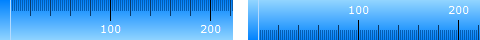
\includegraphics{images/ruler-flipped.png}
\caption{\label{fig:unnamed-chunk-2}The horizontal ruler flipped in both directions.}
\end{figure}

The hatch marks on the ruler can be flipped to be displayed on the opposite side of the ruler.
This is done by pressing the \texttt{Ctrl\ +\ Shift\ +\ Alt\ +\ E} key combination or by the \texttt{Ruler\ Menu\ →\ Flip\ Direction} menu item.
This is assignable to a mouse button click via the \texttt{Flip} function.

\hypertarget{shifttocursor}{%
\section{Shifting to the cursor}\label{shifttocursor}}

The ruler can be shifted to the cursor position using the \texttt{Ctrl\ +\ Shift\ +\ Alt\ +\ S} key combination.
This will shift the ruler along its current axis and position the 0 on the ruler to the cursor position.
Holding down the key will continuously shift the ruler to the cursor position.

\hypertarget{freeze}{%
\section{Freezing the Cursor}\label{freeze}}

You can freeze the cursor on the ruler so that it does not move with the mouse.
This is done by pressing the \texttt{Ctrl\ +\ Shift\ +\ Alt\ +\ F} key combination.

\hypertarget{exit}{%
\section{Exiting the software}\label{exit}}

Exit the software by pressing the \texttt{Ctrl\ +\ Shift\ +\ Alt\ +\ X} key combination or via the \texttt{Ruler\ Menu\ →\ Exit} menu item.

\hypertarget{help}{%
\section{Accessing this help}\label{help}}

You can access this help guide by pressing \texttt{F1} when the ruler is focused or vua the \texttt{Ruler\ Menu\ →\ Help} menu item.

\hypertarget{guidelines}{%
\chapter{Guidelines}\label{guidelines}}

Guidelines allow you to mark specific points on the ruler.
These points can then be \emph{locked on to} with the mouse and allow you to move the mouse along the locked axis.

\hypertarget{adding-and-removing-guidelines}{%
\section{Adding and Removing Guidelines}\label{adding-and-removing-guidelines}}

Add and remove Guidelines by using the \texttt{Ruler\ Menu\ →\ Guidelines}submenu or via the \emph{Guidelines} dialog.
Adding a Guideline will add a new guideline at the current cursor position on the ruler.
Removing a Guideline will remove the nearest guideline to the current cursor position.

\begin{quote}
Both these functions can be assigned to a mouse button.
\end{quote}

\hypertarget{clearing-guidelines}{%
\section{Clearing Guidelines}\label{clearing-guidelines}}

All the Guidelines can be cleared by using the \texttt{Ruler\ Menu\ →\ Guidelines\ →\ Clear\ All} submenu or via the \emph{Guidelines} dialog.
Guidelines are also cleared before Import.

\hypertarget{locking-to-guidelines}{%
\section{Locking to Guidelines}\label{locking-to-guidelines}}

\hypertarget{importing-and-exporting-guidelines}{%
\section{Importing and Exporting Guidelines}\label{importing-and-exporting-guidelines}}

You can import and export Guidelines by using the \texttt{Ruler\ Menu\ →\ Guidelines\ →\ Import} or the \texttt{Ruler\ Menu\ →\ Guidelines\ →\ Export} submenus or via the \emph{Guidelines} dialog.
Either of these options will display a File dialog so that you can select the file to load or save.

\begin{quote}
Importing Guidelines will overwrite any existing Guidelines on the ruler.
\end{quote}

\hypertarget{guideline-file-format}{%
\subsection{Guideline File Format}\label{guideline-file-format}}

Guidelines can be exported to/imported from a simple text file.
The file contains a list of numbers which denote the Guideline pixel position on the ruler.
These files have no preferred extension.

\begin{verbatim}
20
100
150
620
\end{verbatim}

\hypertarget{guideline-dialog}{%
\section{Guideline dialog}\label{guideline-dialog}}

\begin{figure}
\centering
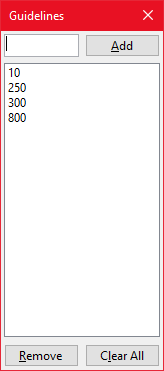
\includegraphics{images/guideline-dialog.png}
\caption{\label{fig:unnamed-chunk-3}The Guideline dialog.}
\end{figure}

The Guideline dialog can be accessed via the \texttt{Ruler\ Menu\ →\ Guidelines\ →\ Edit\ Guidelines} submenu.
This Dialog accepts manual input of Guideline positions and can remove specific Guidelines from the list or clear all Guidelines.

\hypertarget{keyboard}{%
\chapter{Keyboard Shortcuts}\label{keyboard}}

\hypertarget{global-shortcuts}{%
\section{Global Shortcuts}\label{global-shortcuts}}

These shortcuts can be used even when the Screen Pixel Ruler is not focused.

\begin{longtable}[]{@{}ll@{}}
\toprule
\begin{minipage}[b]{0.27\columnwidth}\raggedright
Keystroke\strut
\end{minipage} & \begin{minipage}[b]{0.68\columnwidth}\raggedright
Function\strut
\end{minipage}\tabularnewline
\midrule
\endhead
\begin{minipage}[t]{0.27\columnwidth}\raggedright
Ctrl + Shift + Alt + R\strut
\end{minipage} & \begin{minipage}[t]{0.68\columnwidth}\raggedright
Change ruler rotation.\strut
\end{minipage}\tabularnewline
\begin{minipage}[t]{0.27\columnwidth}\raggedright
Ctrl + Shift + Alt + E\strut
\end{minipage} & \begin{minipage}[t]{0.68\columnwidth}\raggedright
Flip ruler notch direction.\strut
\end{minipage}\tabularnewline
\begin{minipage}[t]{0.27\columnwidth}\raggedright
Ctrl + Shift + Alt + F\strut
\end{minipage} & \begin{minipage}[t]{0.68\columnwidth}\raggedright
Freeze the position marker on the ruler.\strut
\end{minipage}\tabularnewline
\begin{minipage}[t]{0.27\columnwidth}\raggedright
Ctrl + Shift + Alt + S\strut
\end{minipage} & \begin{minipage}[t]{0.68\columnwidth}\raggedright
Move position 0 of the ruler to the current mouse position.\strut
\end{minipage}\tabularnewline
\begin{minipage}[t]{0.27\columnwidth}\raggedright
Ctrl + Shift + Alt + X\strut
\end{minipage} & \begin{minipage}[t]{0.68\columnwidth}\raggedright
Exit Screen Pixel Ruler 2.\strut
\end{minipage}\tabularnewline
\begin{minipage}[t]{0.27\columnwidth}\raggedright
Ctrl + Shift + Alt + A\strut
\end{minipage} & \begin{minipage}[t]{0.68\columnwidth}\raggedright
Add Guideline at current position on the ruler.\strut
\end{minipage}\tabularnewline
\begin{minipage}[t]{0.27\columnwidth}\raggedright
Ctrl + Shift + Alt + D\strut
\end{minipage} & \begin{minipage}[t]{0.68\columnwidth}\raggedright
Delete nearest Guideline from current position on the ruler.\strut
\end{minipage}\tabularnewline
\begin{minipage}[t]{0.27\columnwidth}\raggedright
Ctrl + Shift + Alt + G\strut
\end{minipage} & \begin{minipage}[t]{0.68\columnwidth}\raggedright
Lock mouse position to nearest Guideline.\strut
\end{minipage}\tabularnewline
\bottomrule
\end{longtable}

\hypertarget{local-shortcuts}{%
\section{Local Shortcuts}\label{local-shortcuts}}

These shortcuts only work when the Screen Pixel Ruler has focus.

\begin{longtable}[]{@{}ll@{}}
\toprule
Keystroke & Function\tabularnewline
\midrule
\endhead
F1 & Opens this help guide.\tabularnewline
\bottomrule
\end{longtable}

\hypertarget{config}{%
\chapter{Configuration}\label{config}}

You can access the configuration by right clicking the ruler and selecting \emph{Options}.
This will then display the \emph{Options window} where you can change the configuration.

\begin{figure}
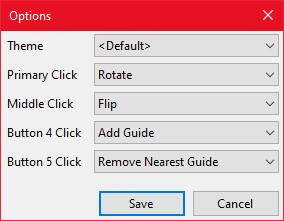
\includegraphics[width=1\linewidth]{images/options} \caption{The options window.}\label{fig:unnamed-chunk-4}
\end{figure}

\hypertarget{options}{%
\section{Options}\label{options}}

\hypertarget{theme}{%
\subsection{Theme}\label{theme}}

Allows you to change the \protect\hyperlink{themes}{theme} of the ruler.

\hypertarget{mouse-button-clicks}{%
\subsection{Mouse button clicks}\label{mouse-button-clicks}}

Allows you to assign mouse button clicking the ruler to specific functionality.
Supports the Primary, Middle, Button 4, and Button 5 mouse buttons.
The following functions are assignable:
- None \emph{Do nothing for the mouse button.}
- Rotate \emph{Rotates the ruler.}
- Flip \emph{Flips the ruler.}
- Add Guide \emph{Adds a guideline to the ruler.}
- Toggle Guide \emph{Toggles the guideline at the current cursor position.}
- Remove Nearest Guide \emph{Removes the nearest guideline to the cursor.}
- Remove All Guides \emph{Removes all guidelines.}
- Lock to Nearest Guide \emph{Locks the mouse to the nearest guideline to the cursor.}

\begin{quote}
Pressing and holding the primary mouse button will always allow you to move the ruler.
\end{quote}

\begin{quote}
The primary mouse button is determined by the \emph{Select your primary button} option in the \emph{Mouse Settings} in Microsoft Windows.
\end{quote}

\hypertarget{location}{%
\section{Location}\label{location}}

Configuration is stored in two locations depending on if you installed from the installer or from the chocolatey package.

Installer: \%appdata\%\textbackslash screenpixelruler\textbackslash app.cfg\\
Chocolatey: \%chocolateyinstall\%\textbackslash lib\textbackslash screenpixelruler\textbackslash tools\textbackslash app.cfg

\hypertarget{themes}{%
\chapter{Themes}\label{themes}}

Themes can change the ruler colour, size or even the interval of the hatch marks.
Screen Pixel Ruler comes with some supplied themes.

\hypertarget{supplied-themes}{%
\section{Supplied Themes}\label{supplied-themes}}

\hypertarget{default}{%
\subsection{Default}\label{default}}

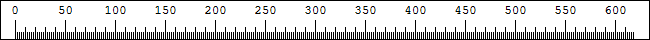
\includegraphics{images/theme-default.png}

A simple black and white theme with a thin ruler.
The built-in default theme.

\hypertarget{panda}{%
\subsection{Panda}\label{panda}}

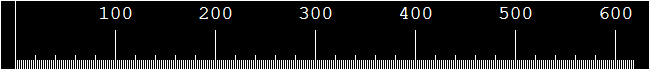
\includegraphics{images/theme-panda.png}

A high contrast theme with a thick ruler for easy visibility.

\hypertarget{mioplanet-pixelruler}{%
\subsection{MioPlanet PixelRuler}\label{mioplanet-pixelruler}}


\includegraphics{images/theme-mioplanet.png}

A blue gradient ruled designed to mimic the look of the MioPlanet PixelRuler software.

\hypertarget{white-chocolate}{%
\subsection{White Chocolate}\label{white-chocolate}}

A white on brown coloured theme.
Simple pallet swap of the Default theme.

\hypertarget{location-1}{%
\section{Location}\label{location-1}}

Themes are stored in the two locations, depending on if you installed from the installer or from the chocolatey package.

Installer: \%appdata\%\textbackslash screenpixelruler\\
Chocolatey: \%chocolateyinstall\%\textbackslash lib\textbackslash screenpixelruler\textbackslash tools

\hypertarget{creating-a-theme}{%
\section{Creating a Theme}\label{creating-a-theme}}

You can create your own themes for Screen Pixel Ruler.
Themes have a \texttt{thm} file extension and are written in \href{https://yaml.org}{yaml}.

\hypertarget{objects}{%
\subsection{Objects}\label{objects}}

Below are objects and explainations of them that can be used in the theme file.

\texttt{\textless{}string\textgreater{}} A string of text.

\texttt{\textless{}boolean\textgreater{}} Either \texttt{true} or \texttt{false}.

\texttt{\textless{}decimal\textgreater{}} A decimal number like \texttt{1.0} or \texttt{1.5}.

\texttt{\textless{}number\textgreater{}} A number like \texttt{1} or \texttt{15}.

\texttt{\textless{}array\textgreater{}} An array of objects.

\texttt{\textless{}colour\textgreater{}} A colour value.
Supported input types are:
- \texttt{\textquotesingle{}\#RRGGBB\textquotesingle{}} Hex/HTML Colour
- \texttt{RRR,\ GGG,\ BBB} Decimal (0-255)
- \texttt{ColorName} Name

\texttt{\textless{}colours\textgreater{}} An array of either one (\texttt{{[}\ \textless{}colour\textgreater{}\ {]}}) or two colour values (\texttt{{[}\ \textless{}colour\textgreater{},\ \textless{}colour\textgreater{}\ {]}}).
If two colours are provided then the colour will be a gradient.

\begin{quote}
For a list of colour names see the \href{https://docs.microsoft.com/en-us/dotnet/api/system.drawing.knowncolor?view=netcore-3.1}{KnownColor Enum} reference.
\end{quote}

\hypertarget{file-format}{%
\subsection{File Format}\label{file-format}}

The rendering order of the elements are \texttt{Background\ ←\ Border\ ←\ Hatch\ Marks\ ←\ Guidelines\ ←\ Cursor}.

\hypertarget{fields}{%
\subsubsection{Fields}\label{fields}}

\begin{verbatim}
Name: <string> The name of the theme.
Cursor: Cursor themeing.
  Line: <colour> The cursor line colour.
  Font: The font used for the cursor.
    Family: <string> The font family.
    Size: <decimal> The font size.
    Bold: <boolean> Whether the font is bold.
    Italic: <boolean> Whether the font is italicised.
    Underline: <boolean> Whether the font is underlined.
    Strikeout: <boolean> Whether the font is striked out.
  Background: <colours> The background colours for the cursor.
  Frozen: The frozen colours for the cursor.
    Line: <colour> The frozen line colour.
    Font: The font used for the frozen cursor.
      Family: <string> The font family.
      Size: <decimal> The font size.
      Bold: <boolean> Whether the font is bold.
      Italic: <boolean> Whether the font is italicised.
      Underline: <boolean> Whether the font is underlined.
      Strikeout: <boolean> Whether the font is striked out.
    Background: <colours> The frozen background colours.
  Locked: The guideline locked colours for the cursor.
    Line: <colour> The locked line colour.
    Font: The font used for the locked cursor.
      Family: <string> The font family.
      Size: <decimal> The font size.
      Bold: <boolean> Whether the font is bold.
      Italic: <boolean> Whether the font is italicised.
      Underline: <boolean> Whether the font is underlined.
      Strikeout: <boolean> Whether the font is striked out.
    Background: <colours> The locked background colours.
Ruler: Ruler themeing.
  Size: <number> The size of the ruler in pixels.
  Background: <colours> The background colour for the ruler.
  Border:
    Colour: <colour> The border colour.
    Spacing: <number> The spacing between the border and the ruler.
  Marks: The hatch marks.
    Colour: <colour> The colour of the hatch marks.
    Size:
      Horizontal: <number> The size of the hatch marks when horizontal.
      Vertical: <number> The size of the hatch marks when vertical.
    Zero: The zero hatch mark.
        NumberVisible: <boolean> Whether the number zero is displayed.
        Size:
          Horizontal: <number> The size of the zero hatch mark when horizontal.
          Vertical: <number> The size of the zero hatch mark when vertical.
    Sizes: <array> The sizes of the hatch marks.
      Interval: <number> The interval of the hatch marks.
      Colour: <colour> The colour of the hatch marks.
      Size:
        Horizontal: <number> The size of the hatch marks when horizontal.
        Vertical: <number> The size of the hatch marks when vertical.
  Numbers: The numbers on the ruler.
    Padding:
      Horizontal: <number> The padding on the left and right of the numbers.
      Vertical: <number> The padding on the top and bottom of the numbers.
    Colour: <colour> The colour of the numbers.
    Font: The font used for the numbers.
      Family: <string> The font family.
      Size: <decimal> The font size.
      Bold: <boolean> Whether the font is bold.
      Italic: <boolean> Whether the font is italicised.
      Underline: <boolean> Whether the font is underlined.
      Strikeout: <boolean> Whether the font is striked out.
    Display:
      Interval: <number> The interval at which numbers should appear.
  Guidelines:
    Guideline: The guidelines.
      Colour: <colour> The colour of the guidelines.
      Size:
        Horizontal: <number> The size of the guidelines when horizontal.
        Vertical: <number> The size of the guidelines when vertical.
    Locked: The guideline locked onto.
      Colour: <colour> The colour of the guideline that has been locked onto.
      Size:
        Horizontal: <number> The size of the guideline that has been locked onto when horizontal.
        Vertical: <number> The size of the guideline that has been locked onto when vertical.
    Nearest: The guideline nearest to the cursor.
      Colour: <colour> The colour of the nearest guideline.
      Size:
        Horizontal: <number> The size of the nearest guideline when horizontal.
        Vertical: <number> The size of the nearest guideline when vertical.
\end{verbatim}

\hypertarget{visual-guide}{%
\subsubsection{Visual Guide}\label{visual-guide}}

\begin{figure}
\centering
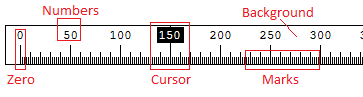
\includegraphics{images/ruler-theme.png}
\caption{\label{fig:unnamed-chunk-8}The Ruler user interface with theme elements highlighted.}
\end{figure}

Zero is the Zero Mark which is explained further below.

Numbers are configured in \texttt{Ruler\ →\ Number} secion.
The \texttt{Ruler\ →\ Number\ →\ Display\ →\ Interval} determines how often the numbers appear.
An interval of \texttt{50} means that numbers will appear at the 50th, 100th, 150th, etc hatch marks.
The other properties under \texttt{Ruler\ →\ Number} determine the font, colour and size of the numbers.

Cursor is the position of the mouse cursor on screen.
Fruther explaination below.

Background is the background colour of the ruler.
This is set at \texttt{Ruler\ →\ Background} and can be a single colour or a gradient when two colours are provided.

\begin{figure}
\centering
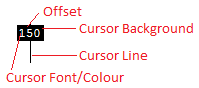
\includegraphics{images/ruler-cursor.png}
\caption{\label{fig:unnamed-chunk-9}The cursor that appears in the ruler.}
\end{figure}

The above options are all configured in the \texttt{Cursor} section.
\texttt{Cursor\ →\ Frozen} is used when the cursor is \protect\hyperlink{freeze}{frozen}.

\begin{figure}
\centering
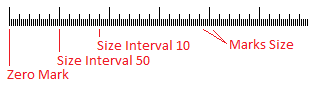
\includegraphics{images/ruler-hashmarks.png}
\caption{\label{fig:unnamed-chunk-10}The ruler hatch marks.}
\end{figure}

\emph{Zero Mark} hatch mark is provided by the \texttt{Ruler\ →\ Marks\ →\ Zero\ →\ Size} property.
You can also set the \texttt{Ruler\ →\ Marks\ →\ Zero\ →\ NumberVisible} property to \texttt{false} to omit the 0 number.

Size interval 10 and Size Interval 50 hatch marks are provided by the \texttt{Ruler\ →\ Marks\ →\ Sizes} array.
Below is an example of a 50 pixel interval hatch mark:

\begin{Shaded}
\begin{Highlighting}[]
\CommentTok{...}
\CommentTok{  Marks:}
\CommentTok{    Sizes:}
\CommentTok{      - Interval: 50}
\CommentTok{        Colour: #000000}
\CommentTok{        Size:}
\CommentTok{          Horizontal: 20}
\CommentTok{          Vertical: 40}
\CommentTok{...}
\end{Highlighting}
\end{Shaded}

\emph{Marks Size} hatch marks are provided by the \texttt{Ruler\ →\ Marks\ →\ Size} properties.
The colour is provided by the \texttt{Ruler\ →\ Marks\ →\ Colour} property.
Every even pixel on the ruler will have a hatch mark provided by this value.
Set the size to \texttt{0} to omit the default hatch marks.

\hypertarget{default-values}{%
\subsubsection{Default Values}\label{default-values}}

Font\\
\hspace*{0.333em}\hspace*{0.333em}\hspace*{0.333em}\hspace*{0.333em}Family: \texttt{Courier\ New}\\
\hspace*{0.333em}\hspace*{0.333em}\hspace*{0.333em}\hspace*{0.333em}Size: \texttt{9}\\
\hspace*{0.333em}\hspace*{0.333em}\hspace*{0.333em}\hspace*{0.333em}Bold: \texttt{false}\\
\hspace*{0.333em}\hspace*{0.333em}\hspace*{0.333em}\hspace*{0.333em}Italic: \texttt{false}\\
\hspace*{0.333em}\hspace*{0.333em}\hspace*{0.333em}\hspace*{0.333em}Underline: \texttt{false}\\
\hspace*{0.333em}\hspace*{0.333em}\hspace*{0.333em}\hspace*{0.333em}Strikeout: \texttt{false}\\
~\\
Cursor → Locked\\
\hspace*{0.333em}\hspace*{0.333em}\hspace*{0.333em}\hspace*{0.333em}Cursor → Frozen\\
~\\
Cursor → Frozen\\
\hspace*{0.333em}\hspace*{0.333em}\hspace*{0.333em}\hspace*{0.333em}Cursor\\
~\\
Ruler → Background\\
\hspace*{0.333em}\hspace*{0.333em}\hspace*{0.333em}\hspace*{0.333em}\hspace*{0.333em}\texttt{White}\\
~\\
Ruler → Marks → Zero → NumberVisible\\
\hspace*{0.333em}\hspace*{0.333em}\hspace*{0.333em}\hspace*{0.333em}\texttt{false}\\
~\\
Ruler → Marks → Zero → Colour\\
\hspace*{0.333em}\hspace*{0.333em}\hspace*{0.333em}\hspace*{0.333em}Ruler → Marks → Colour\\
\hspace*{0.333em}\hspace*{0.333em}\hspace*{0.333em}\hspace*{0.333em}\hspace*{0.333em}\hspace*{0.333em}\hspace*{0.333em}\hspace*{0.333em}\texttt{Transparent}\\
~\\
Ruler → Guidelines → Nearest\\
\hspace*{0.333em}\hspace*{0.333em}\hspace*{0.333em}\hspace*{0.333em}Ruler → Guidelines → Guideline\\
~\\
Ruler → Guidelines → Locked\\
\hspace*{0.333em}\hspace*{0.333em}\hspace*{0.333em}\hspace*{0.333em}Ruler → Guidelines → Guideline\\
~\\
Ruler → Guideline → Guideline → Size\\
\hspace*{0.333em}\hspace*{0.333em}\hspace*{0.333em}\hspace*{0.333em}\hspace*{0.333em}Ruler → Size\\
~\\
Ruler → Guideline → Guideline → Colour\\
\hspace*{0.333em}\hspace*{0.333em}\hspace*{0.333em}\hspace*{0.333em}\hspace*{0.333em}Ruler → Marks → Colour

\end{document}
